\documentclass[conference]{IEEEtran}
\usepackage{times}

% numbers option provides compact numerical references in the text. 
\usepackage[numbers]{natbib}
\usepackage{multicol}
\usepackage[bookmarks=true]{hyperref}
\usepackage{graphicx}
\usepackage{amsmath,amsfonts,amssymb}
\usepackage{hyperref}

\graphicspath{ {./graphics/} }

\pdfinfo{
   /Author (Mingyo Seo)
   /Title  (Robots: Our new overlords)
   /CreationDate (D:20101201120000)
   /Subject (Robots)
   /Keywords (Robots;Overlords)
}

\begin{document}

% paper title
\title{CS391L HW4: Gaussian Process}

% You will get a Paper-ID when submitting a pdf file to the conference system
\author{Mingyo Seo}

\author{\authorblockN{Mingyo Seo}
\authorblockA{
UT EID: ms84662\\
Email: mingyo@utexas.edu}}



\maketitle

\IEEEpeerreviewmaketitle

\begin{abstract}
In this assignment, an overview of Gaussian processes (GP) is presented and is applied to estimate a trajectory from human motions.
I used a dataset of 5 different iterations of the same motion and mixed signals to generate a single trajectory.
In particular, I used an exponent RBF kernel for trajectory processing.
The regression was implemented by the gradient ascent algorithm to maximize the negative log-likelihood function, which outputs the optimal kernel hyperparameters.
I also compared the use of a single global GP and a set of GP's fit to local data and studied how the local GP's hyperparameters change.
\end{abstract}

\section{Introduction} % Introduce your problem and the overall plan for approaching your problem

The problem of estimating a trajectory from multiple demonstrations can be applied to many areas.
In this paper, in particular, I implemented a Gaussian process(GP) model to estimate a trajectory from human demonstration. 
GP is one of the statistical parameter-free models.
By using a GP model, we can predict and estimate a likelihood at any given dataset.
We can consider a GP as a multi-dimensional Gaussian Probability density function (PDF).
A GP is characterized by a set of mean and variance functions.
By sampling a finite or infinite-dimensional PDF, we can regress the mean and variance functions, which is formulated as,
\begin{equation}
\begin{aligned}
    f \in \mathcal{N}(\mu(\boldsymbol{x}),V(\boldsymbol{x}))\ \text{sampled from PDF},\\
    \text{where} \quad \mu \in R^n,\ V\in R^n\times R^n.
\end{aligned}
\end{equation}
For the implementation of GP, I used mixed motion demonstration data from multiple datasets to estimate a motion trajectory.

The answers to the HW4 questions are included in the following sections.
\begin{itemize}
\item Fig. \ref{fig:global}: Pridiction of the motion data using a global kernel
\item Fig. \ref{fig:local}: Prediction of motion data using local kernels
\item Fig. \ref{fig:likelihood}, \ref{fig:square_error}: Performances of the global/local kernels
\item Fig. \ref{fig:hyper}: Hyperparameter of local kernels at each frame 
\item Tab. \ref{table:interval}: Intervals where the kernels cluster with similar\\
\quad values
\end{itemize}


\section{Method}
\label{sec:method}

\subsection{Finite Gaussian Process}
We assume that the prior distribution follows a Gaussian distribution of the mean($m_f$) and ithe dentity co-variance matrix($K_{ff}$), represented as,
\begin{equation}
\begin{aligned}
    &\quad f(\boldsymbol{x})\ \sim \ GP(m(x),\kappa(x,x')) \Leftrightarrow f \in \mathcal{N}(m_f,K_{ff}),
\end{aligned}
\end{equation}
where
\begin{equation}
\begin{aligned}
    &m(x) = \mathbb{E}[f(x)]\\
    &\kappa(x,x') = \mathbb{E}[(f(x)-m(x))(f(x')-m(x'))].
\end{aligned}
\end{equation}
Thus, we can update the posterior from a data $(X, y)$
By using Bayes' theorem, the GP is represented as,\\
\begin{equation}
\begin{aligned}
    &P(f|y)\\ 
    &\quad = \mathcal{N}(K_{fy}^TK_{yy}^{-1}(y-m_y) +m_f, K_{ff}-K_{fy}^TK_{yy}^{-1}K_{fy}^T).
\end{aligned}
\end{equation}
The above formulas exist in an infinite dimensional space. 

To apply the form of an infinite GP into a finite data set, we reformulate the GP formulation and use a Kernel function to calculate the co-variance matrix. 
If the optimal GP of the finite data set $(X,y)$ is given by $f$, then predictions for new data $X_*$ given by $f_*$ are given as,
\begin{equation}
\begin{aligned}
    \begin{bmatrix}
    f\\
    f_*
    \end{bmatrix} = \mathcal{N}\left( 0, \begin{bmatrix}
    K(X,X)\    K(X,X_*)\\
    K(X_*,X)\    K(X_*,X_*)
     \end{bmatrix}    
    \right)
    \label{eq:Ensemble}
\end{aligned}
\end{equation}
Instead of sampling multiple $f_*$ from the ensemble of equation \ref{eq:Ensemble}, we can condition our prior of $f$ for $(X,y)$. 
If there is no noise in the observed output $y$, then the best solution is $f=y$, and
\begin{equation}
\begin{aligned}
    f_*|X_*,X,f & \\
    \sim \mathcal{N} (& K(X_*,X)K(X,X)^{-1}f, \\
    & K(X_*,X_*)- K(X_*,X)K(X,X)^{-1}K(X,X_*)) 
    \label{eq:fstar}
\end{aligned}
\end{equation}
In particular, we use an exponent RBF kernel to calculate the co-variance matrix $K$ and Gaussian noise to estimate raw data errors, given as
\begin{equation}
\begin{aligned}
    &y(u) = f(u) + \epsilon\\
    &k(u_i,u_j) = e^{\sigma_f}e^{\left(\frac{1}{2}e^{\sigma_l}||u_i-u_j||^2\right)} \\
    &q(u_i,u_j) = k(u_i,u_j) + e^{\sigma_n}\delta_{ij},
    \label{eq:Kernel with noise}
\end{aligned}
\end{equation}
where $\epsilon \sim \mathcal{N}(0,e^{\sigma_n}).$
This also can be written as, 
\begin{equation}
\begin{aligned}
Q(X,X) = K(X,X) + e^{\sigma_n}I_{n\times n}.
\end{aligned}
\end{equation}
Then, we can estimate $f_*$ for new values $X_*$ using equation \ref{eq:fstar}, as
\begin{equation}
\begin{aligned}
    &\Bar{f_*} = K(X_*,X)K(X,X)^{-1}y\\
    &\mathbb{V}[f_*] = K(X_*,X_*) - K(X_*,X)Q(X,X)^{-1}K(X,X_*),
\end{aligned}
\end{equation}
where $K(X_*,X) = \left[K(X,X_*)\right]^T$.
The variance at each $x_*$ is given by the diagonal elements of $\mathbb{V}[f_*]$. 
The standard deviations from these values can be used to compute the 95\% confidence interval at each $x_*$.
Also, from $f_*$, we can calculate the expectation and variance of the observations $y_*$. Since adding white noise does not change mean observation, the mean is given as,
\begin{equation}
\begin{aligned}
    \Bar{y_*} = \Bar{f_*}.
\end{aligned}
\end{equation}
The variance is given as
\begin{equation}
\begin{aligned}
	\mathbb{V}[y_*] = Q(X_*,X_*) - K(X_*,X)Q(X,X)^{-1}K(X,X_*).
\end{aligned}
\end{equation}


\subsection{GP Hyperparameter regression}

A regression on the hyper-parameters, $\sigma = [\sigma_f,\sigma_l,\sigma_n]$ obtains the optimal GP over the given data. 
Consider the log-likelihood function, given as 
\begin{equation}
\begin{aligned}
    log P(y|x,\sigma) = -\frac{1}{2}y^TQ^{-1}y - -\frac{1}{2}log(det(Q)) - \frac{n}{2}log(2\pi)
     \label{eq:logP}
\end{aligned}
\end{equation}
The GP regression can be processed by maximizing the log-likelihood function \cite{bishop}, as 
\begin{equation}
\begin{aligned}
	\sigma_{i+1} = \sigma_{i} + \eta\cdot
	\left[ {\nabla}_\sigma (log P) \right]_{\sigma_i}.
	\label{eq:gradient ascent}
\end{aligned}
\end{equation}
Here, $\eta$ is the vector learning rate.
Then, the gradient of the $logP$ function is given by:
\begin{equation}
\begin{aligned}
    {\nabla}_\sigma(log P) = -\frac{1}{2}y^T\frac{\partial Q^{-1}}{\partial \Vec{\sigma}}y - -\frac{1}{2}\frac{\partial log(|Q|)}{\partial \Vec{\sigma}},
\end{aligned}
\end{equation}
where
\begin{equation}
\begin{aligned}
    &\frac{\partial log(|Q|)}{\partial {\sigma}} = trace\left( Q^{-1}\frac{\partial Q}{\partial {\sigma}}\right)\\
    &\frac{\partial Q^{-1}}{\partial {\sigma}} = -Q^{-1} \frac{\partial Q}{\partial {\sigma}} Q^{-1},
\end{aligned}
\end{equation}    
and the partial differentials are given as,
\begin{equation}
\begin{aligned}
    &\frac{\partial Q_{ij}}{\partial \sigma_f} = K_{ij}\\
    &\frac{\partial Q_{ij}}{\partial \sigma_l} = K_{ij}\times \left(-\frac{1}{2}e^{\sigma_l}||x_i-x_j||^2 \right)\\
    &\frac{\partial Q}{\partial \sigma_n} = e^{\sigma_l}I.
\end{aligned}
\end{equation}

\section{Results} % Describe the methods you intend to apply to solve the given problem

In the assignment, I trained the GP model to estimate the trajectory from multiple demonstrations of the same task. 
For the training process, I used the learning rate $\eta=0.01$ and the finite time-horizon of 50 frames. 
For moving windows, I used the 5-frame stride.
The set of the kernel hyperparameters was used for the initialization.
\begin{equation}
\begin{aligned}
\sigma_f &= -1.9496\\
\sigma_l &= -13.837\\
\sigma_n &= -6.6605.
\end{aligned}
\end{equation}

For regression, I limited the maximum iteration of gradient ascent under $2,000$.
To avoid divergence, I also terminated the gradient ascent process at each window if the magnitude of the gradient reached the limit under 1, as
\begin{equation}
\begin{aligned}
	|| \left[ {\nabla}_\sigma (log P) \right]_{\sigma_i}  || < 1.
	\label{eq:gradient ascent}
\end{aligned}
\end{equation}

In this assignment, I used the dataset of Subject \textit{YY} and Marker \textit{14\_x}.
To avoid the effects of the raw data noise, we mixed the 5 demonstrations to generate a single trace data.

\subsection{Kernels}

\begin{figure}[!t]
	\centering
	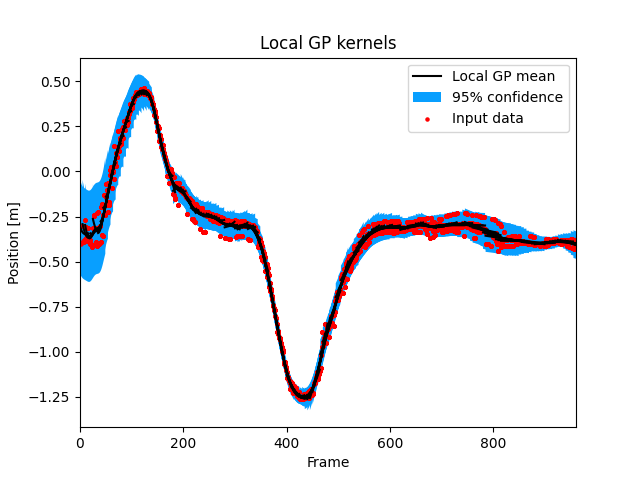
\includegraphics[width=3.6in]{local.png}	
	\caption{Visualization of the local GP model at Subject \textit{YY} and Marker \textit{14\_x}.}
	\label{fig:local}
\end{figure}


\begin{figure}[!t]
	\centering
	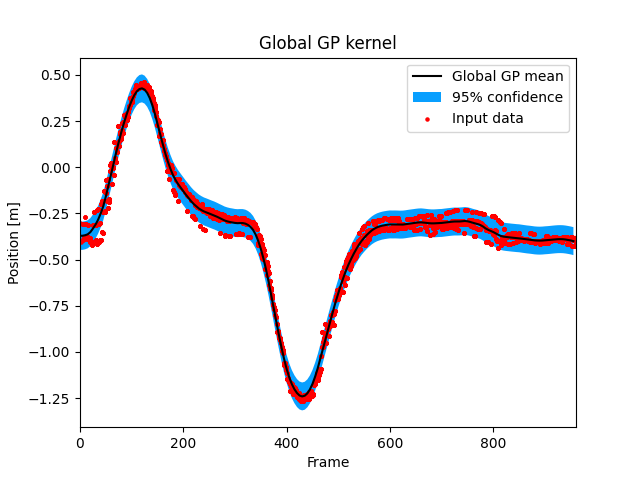
\includegraphics[width=3.6in]{global.png}	
	\caption{Visualization of the global GP model at Subject \textit{YY} and Marker \textit{14\_x}.}
	\label{fig:global}
\end{figure}

The GP model with the local kernel is presented in Figure \ref{fig:local}.
The GP model with the global kernel is presented in Figure \ref{fig:global}.
The optimal set of the hyperparameters used in the global kernel were computed as below,
\begin{equation}
\begin{aligned}
\sigma_f &= -2.6004\\
\sigma_l &= -12.206\\
\sigma_n &= -6.5438.
\end{aligned}
\end{equation}

\begin{figure}[!t]
	\centering
	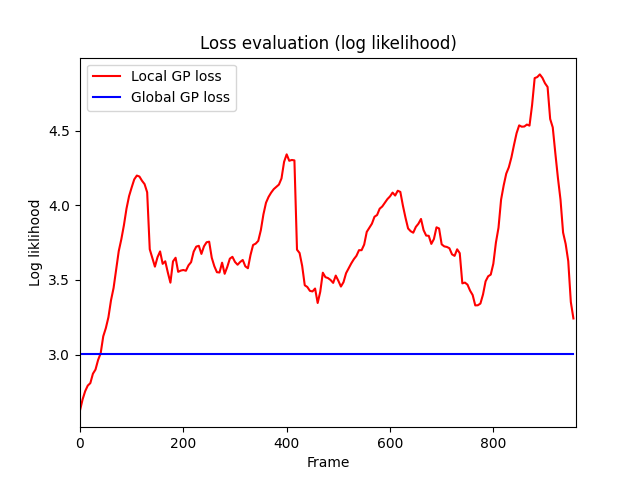
\includegraphics[width=3.6in]{log_likelihood.png}	
	\caption{Log-likelihood comparison between the local and global GPs.}
	\label{fig:likelihood}
\end{figure}

\begin{figure}[!t]
	\centering
	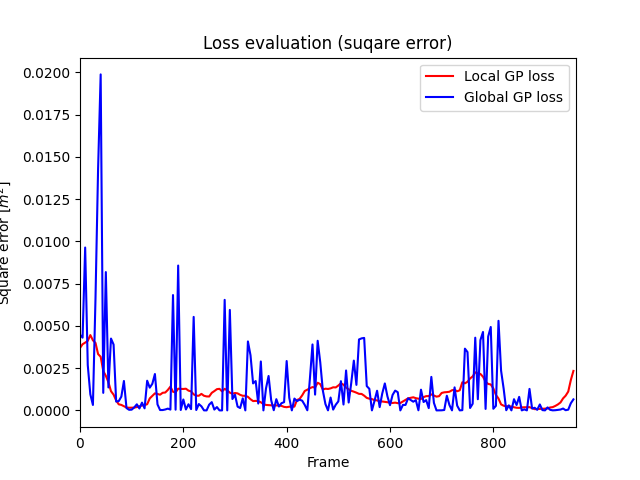
\includegraphics[width=3.6in]{square_error.png}	
	\caption{Square error comparison between the local and global GPs.}
	\label{fig:square_error}
\end{figure}

To compare the performance of the local GP model and the global GP model, I consider two metrics: log-likelihood, the target function of the gradient ascent, and square errors.
The log-likelihood of the models is presented in Figure \ref{fig:likelihood}.
In the plots, the global GP model has high likelihood values at the beginning of the process, but the local GP model shows higher likelihood values in most of the processes.
From this, we can find that the local GP kernel is poorly initialized but becomes fitting well on the dataset as the regression is processed.
On the other hand, from the square errors of the models, as presented in Figure \ref{fig:square_error}, the global GP model has larger variance and magnitude on square errors.
This implies that the globally optimal kernel hyperparameters may not fit on the local data.
Also, the results of better performance in the local GP models imply the correlation of the two different metrics.


\subsection{Hyperparameters}

\begin{figure}[!t]
	\centering
	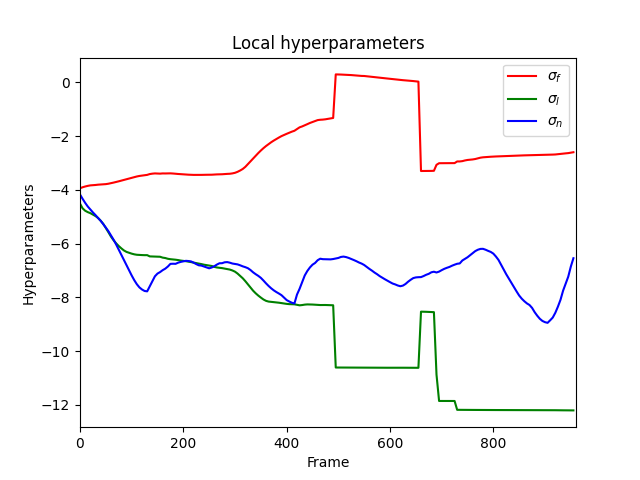
\includegraphics[width=3.6in]{hyper.png}	
	\caption{Hyperparameters of the local GP model.}
	\label{fig:hyper}
\end{figure}


\begin{figure}[!t]
	\centering
	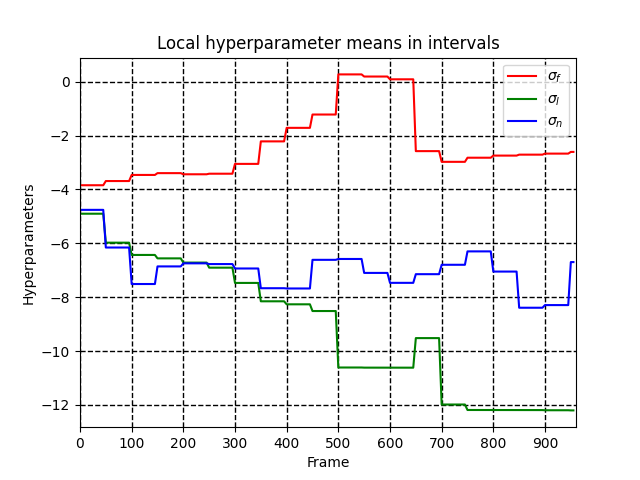
\includegraphics[width=3.6in]{interval.png}	
	\caption{Correlation between each source signal and the corresponding the restored signal}
	\label{fig:interval}
\end{figure}

\begin{table}
\caption{Intervals with similar values}
 	\label{table:interval}
\begin{tabular}{ |p{1.5cm}||p{1.2cm}|p{1cm}|p{1cm}|p{1cm}|  }
 \hline
 Interval ID & Frame & $\sigma_f$ & $\sigma_l$ & $\sigma_n$\\
 \hline
	1 & 0-50 	&		&		&		\\
	2 & 50-100 	&		&		&		\\
	3 & 100-150 & 3-6 	&		&		\\
	4 & 150-200 & 3-6 	& 4-7 	&		\\
	5 & 200-250 & 3-6 	& 4-7 	&		\\
	6 & 250-300 & 3-6 	& 4-7 	&		\\
	7 & 300-350 &		& 4-7 	&		\\
	8 & 350-400 &		&		&		\\
	9 & 400-450 &		&		&		\\
	10 & 450-500 &		& 10-11 &		\\
	11 & 500-550 & 11-13 & 10-11 & 11-13\\
	12 & 550-600 & 11-13 &		& 11-13\\
	13 & 600-650 & 11-13 &		& 11-13\\
	14 & 650-700 &		 &		&		\\
	15 & 700-750 &		 &		&		\\
	16 & 750-800 & 16-20 &		& 16-20 \\
	17 & 800-850 & 16-20 &		& 16-20 \\
	18 & 850-900 & 16-20 & 18-19 & 16-20 \\
	19 & 900-950 & 16-20 & 18-19 & 16-20 \\
	20 & 950-1000 & 16-20 &		& 16-20 \\
 \hline
\end{tabular}
\end{table}

The kernel hyperparameters of the local GP model are presented in Figure \ref{fig:hyper}.
For the analysis of intervals with similar values, I visualized the means of the hyperparameters at each interval in Figure \ref{fig:interval}.
In Table \ref{table:interval}, intervals with similar values are represented with interval IDs.
In particular, we can find that $\sigma_f$ and $\sigma_n$ have shared intervals, which implies those two parameters are correlated. 
Also, in the Interval 18-19 (Frame 850-950), where the trajectory in Figure \ref{fig:local} does not change aggressively, all the parameters have similar values.
From this result, we can confirm that kernel hyperparameters highly depend on the characteristics of trajectories.

\section{Summary} %Intermediate/Preliminary Results: State and evaluate your results upeto the milestone

The GP model and gradient ascent for regressing the model from raw motion data are implemented in the assignment. 
For training, I mixed 5 human motion datasets of the same task demonstration and estimated the trajectory by regressing the GP model.
By the regression, I optimized the optimal set of hyperparameters for the finite GP kernel from the given data.
From the results of the experiments, we can confirm that a sliding window kernel can fit the given data more accurately than a global kernel function.
This is verified by taking the mean of log-likelihood and square errors over all the points it spans.
Also, we confirmed that local kernels have similar hyperparameters when the behavior of the motion data does not change aggressively.
%\section*{Acknowledgments}

%% Use plainnat to work nicely with natbib. 

\bibliographystyle{plainnat}
\begin{thebibliography}{9}
\bibitem{bishop}
Christopher M. Bishop (2006) \emph{Pattern Recognition and Machine Learning}, Springer.
\end{thebibliography}


\end{document}


